%!TEX root = ../../thesis.tex

\section{Discussion}
\label{sec:chisquared_discussion}
The spectral differential and the synthetic recovery methods attempted both in this chapter and \cref{cha:direct_recovery} were both unsuccessful in an actual detection of the {BD} companions focused in this work.
The injection-recovery simulations at a \snr{} of 300 give a companion upper mass limit around \(600^{+20}_{-40}\), above which this method detects a simulated secondary spectra.
This is very high, roughly six times higher then the {BD} mass limit \(\sim\)80--90\Mjup{}.
Some potential reasons and solutions for these poor results are given below, that hopefully can provide some guidance for any future attempts with these methods.

\subsection{Mismatch in synthetic models}
\label{subsec:mismatch}
It is believed that spectral mismatch between the observation and synthetic spectra is the main cause of the unsuccessful companion detection, impacting the recovery in two ways.
The mismatch causes the \textchisquared{} values to be large in general, but this also causes the companion temperature to be pushed to higher temperatures in the application to the real observations.

In the examples shown the \Logg{} and metallicity of the synthetic models are held fixed, leaving only temperature to vary.
The temperature impacts the synthetic spectral models in two main ways: the flux level of the continuum, and the number and strength of the absorption lines.
In the binary model the contributions of the individual components is scaled by the flux ratio.
If the temperature of the companion increases then the flux and radius of the companion increases and the flux ratio \FoneFtwo{} decreases.
This effectively makes the lines in the host component relatively smaller in the normalized binary model spectrum.
Due to the large initial mismatch of synthetic spectral lines of the host, a decrease in the relative strength of the host lines reduces the \textchisquared{} value.
This causes the recovered temperature of the companion to be higher than expected, >2000\K{} higher if allowed by the size of the exploration grid.
The \textchisquared{} approach is dominated by reducing the mismatch in the spectrum of the host rather than detecting the spectra of the companion.
This spectral mismatch is not observed in the simulations in \cref{subsec:simulated_binaries} because they are created using the synthetic spectra themselves, and hence they do not have this same problem with the companion temperature.

\todo{Find the wavelengths of some missing lines in the Mismatch, what elements do they belong to}

Although the newer generations synthetic spectral models are improving and match the overall spectral energy distribution reasonably well there are still regions in the \emph{H}- and \emph{K}-band where there is room for improvement~\citet{rajpurohit_spectral_2016}.
These can come in several forms, such as molecular line lists, abundance measurements, or further modelling.
As one example in particular, \citet{rajpurohit_spectral_2016} previously inferred that the \ce{TiO} line list poorly matches the real positions of \ce{TiO} lines at spectral resolutions of \(\sim\)100\,000.
\citet{passegger_carmenes_2018} has also noted inconsistencies in the line depth of synthetic spectra.
The spectral mismatch in the region studied here is still too large for spectral recovery of companion brown dwarfs.
In the \nir{} there is a compounding problem: the model input physics of sub-stellar temperatures and chemistry combined with the general difficulty of the \nir{}.

\subsection{Line contribution of faint companions}
\label{subsec:line_contributions}
One thing easy to overlook when attempting to detect the binary companion at low flux ratios is the actual contribution of the spectral lines of the companion.
Here the line depths in the synthetic companion spectra are calculated to determine the \snr{} levels required to detect the lines of the binary companions.

The flux ratio of the continuum for the most promising target analysed here is \FtwoFone{}\(\sim\)3\% with the other targets having an expected flux ratio below 1\%.
The spectral lines of the individual components, which are the features that allow the identification and recovery of the components, have depths on average around 10--20\% of their respective continua; at-least between 2110--2160\nm{}.
In effect, the companion line features have a depth \(\ll 1\%\) relative to the continuum of the combined spectrum.

In \cref{tab:line_contributions} some properties of the spectral lines in the {PHOENIX-ACES} library between 2110--2160\nm{} are calculated.
The number of spectral lines (\emph{no.~lines}) deeper than 5\% are counted and the the average depth (\emph{avg.~depth}) of these lines is calculated.
The contribution depth \emph{cont.~depth} of the companion lines to a combined spectrum is calculated to account for the flux ratio between the two spectral components.
Here a Sun-like host with \(\teffsub{1}=5800\)\K{} is used for the comparison.
This simplified combination neglects the continuum shapes of both spectral components and uses the average flux ratios for this wavelength range.
The {PHOENIX-ACES} spectra in the temperature range of 2500--5000\K{} shown in \cref{fig:comp_spectra} can be used to get a visual indication of the line density and depth measured here.

For the lower temperature spectra there are more lines >5\% deep, with 360--460 lines in this wavelength range, compared with only 31 deep absorption lines found in a Sun-like spectrum in this range.
The average line depth of these lines is also larger than the Sun-like spectrum, around twice as deep.
However, when accounting for the flux ratio, the contribution of the companion lines is 1--2 orders of magnitude smaller than the lines of the host.

For example, with the synthetic model for the companion of {HD~211847}, the average contributions of lines >5\% become only 0.3\% deep in a binary with the Sun-like spectrum.
For a companion with a temperature of 2300\K{} (the lower {PHOENIX-ACES} temperature limit) the deepest lines contribute lines only around 0.1\%.

%{\bl We use the contributed line depth values to calculate the \snr{} level required to have Gaussian noise of the same height and the observed \snr{} required to achieve equivalent contribution from all N lines of the spectrum, \(\rm \textrm{SNR}_N = \textrm{SNR} /\sqrt{N}\).
%This is for the synthetic spectra which have many more lines than the observed spectra in this wavelength range.}

The \snr{} of the observed spectra is between 100--300, which is below the \snr{} of 323 needed for the detection of the low-mass star companion of {HD~211847} with temperature of 3200\K{} and \Logg{} 5.0.
For the other targets with {BD} companions at and below the {PHOENIX-ACES} temperature range, a \snr{} >800  would be required to detect the individual spectral lines of the companion.
With the \snr{} increasing with \(\sqrt{N}\) this would require the observational time for each target to be increased by a factor of \(\sim\)10--64.

Our non-detection of binary companions with low flux ratios is consistent with other works.
For example~\citet{nemravova_xtauri_2016} performed extensive spectral analysis of a quadruple-star system \object{$\xi$ Tauri} using 227 spectra in 3 different wavelength bands with \(R=10\,000--48\,000\).
Of the four stars in the system they were unable to detect the spectral component of the star which had a luminosity ratio below 1\%.

%!TEX root = ../nir_companions.tex

\begin{table}
    \small
    \centering
    \begin{threeparttable}[b]
        \caption[Analysis of spectral line depths.]{Contribution of synthetic lines within 2\,110--2\,160\nm{} of synthetic {PHOENIX-ACES} spectra to a binary model. \(F_{2}/F_{1}\) is the continuum flux ratio between a spectrum with the given \Teff{} and \logg{} and a Sun-like spectrum with \(\teff{}=5\,800\),\logg{} = 4.5 (right most column). \emph{No.\ lines} is the number of spectral lines deeper than 5\% from the continuum of the individual spectra while \emph{avg.\ depth} is the mean depth of those lines. \emph{Cont.\ depth} is the average contribution, or depth, of these lines in the combined spectrum of a binary with a Sun-like spectrum. The \snr{} is signal-to-noise level required to have Gaussian noise \(\sigma=1/\snr{}\)  equal to the \emph{cont.\ depth} level in the binary model. All synthetic spectra used here have \feh{}=0.0.}
        \begin{tabular}{*7c}
            \toprule
            \teff{} (K)  & \multicolumn{2}{c}{2300} & \multicolumn{2}{c}{3200} & 5\,800 (\(\rm F_1\))\\
           \logg{} & 5.0 & 4.5  & 5.0 & 4.5 & 4.5 \\
            \midrule
            \(F_2/F_1\) & 0.006 & 0.019 & 0.029  & 0.091 & 1.000 \\
            % {>2\%}  & no. lines & 470 &  463 & 414  & 444 & 111 \\
            % & avg.\ depth & 0.20 & 0.23 & 0.10  & 0.12 & 0.04 \\
            % & cont. depth \tablefootmark{a} & 0.0012 &  0.0043 & 0.0028 &  0.0100 &  0.0333\tablefootmark{b} \\
            % \midrule
            no.\ lines & 464 & 463 & 365  & 413 & 31 \\
            avg.\ depth & 0.2  & 0.23 & 0.11 & 0.12 & 0.10 \\
            cont.\ depth\tnote{a} &  0.0012 & 0.0043 &  0.0031 & 0.0100 &  0.0833\tnote{b} \\
            \snr{}  & 833 & 232 & 323  & 100 & 12 \\
            %  {SNR}\(\rm _N\)  & 39 & 11 & 17  & 5 & 2 \\
            \bottomrule
        \end{tabular}\label{tab:line_contributions}
        \begin{tablenotes}
            \item [a] avg.\ depth \(\times~ \rm F_2 / (F_1 + F_2)\), where \(F_1\) is the component in the far right column.
            \item[b] avg.\ depth \(\times~ \rm F_1 / (F_1 + F_2)\), where \(\rm F_2\) is for the companion with \teff{}=3200, \logg{}=4.5.
        \end{tablenotes}
    \end{threeparttable}
\end{table}



\begin{figure}
    \centering
    %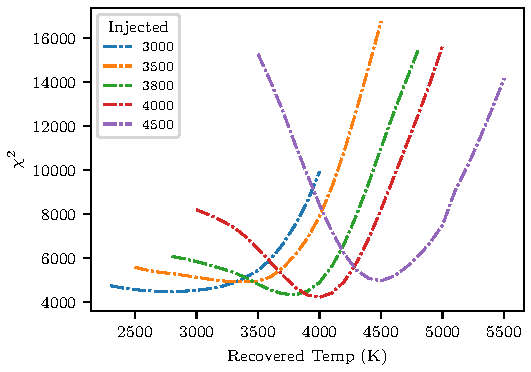
\includegraphics[width=0.7\linewidth]{figures/companion_recovery/chi2_shape_investigation}
    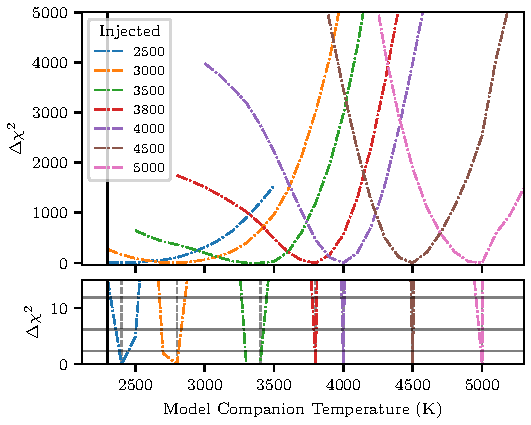
\includegraphics[width=0.7\linewidth]{figures/companion_recovery/chi2_shape_investigation_with_delta}
    \caption[Shape of simulated \textchisquared{} with different injected companion temperatures.]{Top: Companion temperature verses \textchisquared{} for simulations with different injected companion temperatures.
        The other fixed parameters for these fully synthetic simulations was \(\teffsub{1}=5200\)\K{}, \(\logg_{1}=4.5\), \(\logg{}_{2}=5.0\), and both \feh{}=0.0.
        A fixed Gaussian noise corresponding to a \snr{} of 300 was used.
        Bottom: A close up view of \textchisquared{} below 15.
        The three horizontal grey lines indicate the 1-, 2-, 3-$\sigma$ with two degrees of freedom.
        The vertical dotted lines indicate the location of the minimum \textchisquared{} recovered for each companion.
        The black solid vertical in both panels shows the 2300\K{} cut-off of the {PHOENIX-ACES} models}
    \label{fig:injection_shape}
    %\label{fig:chi2shapeinvestigation}
\end{figure}

\todo{}
\subsection{\(\chi^2\) asymmetry} 
\label{subsec:chi2_assymetry}

To try and understand this recovered companions further investigation into the \textchisquared{} space was performed of the {HD30501} synthetic simulation.
The minimum \textchisquared{} contours achieved for each companion temperature in the grid, regardless of \Rvtwo{} are shown in \cref{fig:injection_shape}.
This is done for seven different injected companion temperatures, \(\teffsub{2}\), between 2500 and 4500\K{}.
For the higher temperature companions, the \textchisquared{} is parabolic in shape, recovering the correct temperature, as expected.
At lower temperatures there is a strong asymmetry in the \textchisquared{} with it flattening out on the lower temperature side.
The 1-, 2-, 3-\(\sigma\) values (with two degrees of freedom) of 2, 6 and 11 above the minimum \textchisquared{} are not shown in the bottom panel of \cref{fig:injection_shape} which is a close-up around the minimum \textchisquared{} as they are indistinguishable in the top panel due to the extreme \textchisquared{} y-scale.
The black vertical line indicates the 2300\K{} temperature limit of the {PHOENIX-ACES} models.

In \cref{fig:injection_shape} \textrm{we} showed that the shape of the recovered \textchisquared{} becomes asymmetric when dealing with companion temperatures below around 3800\K{}.
A visual inspection of the spectra reveals the likely cause.
In \cref{fig:comp_spectra} \textrm{we} show the corresponding spectra between 2111--2165\nm{}.
As the temperature decreases the strongest lines become less prominent, disappearing progressively among the other many small lines that appear at lower temperatures.
Hence there are no strong companion lines to easily distinguish one temperature from another.
In the flatter part of the \textchisquared{} curves several low temperature companions are equally well fitted to the simulation/observation.

\cref{fig:injection-recovery,fig:injection_shape} show different recovered temperatures but both agree above 3800\K{}.
A higher companion temperature is recovered between 2800 and 3800\K{}, where as in \cref{fig:injection_shape} a lower temperature is recovered.
This is probably due to a combination of the noise added, and the asymmetries of the \textchisquared{} lines.
\cref{fig:injection-recovery} uses the noise level from the observed spectrum while \cref{fig:injection_shape} has a \snr{} of 300.
This large asymmetry can also explain the jump observed in the synthetic recovery temperature around 2700\K{} in \cref{fig:injection-recovery}.

The asymmetry also causes an asymmetry in the \textchisquared{} error bars which can be seen in the bottom panel of \cref{fig:injection_shape}.
For instance the recovered value and 1-\(\sigma\) error bars on the 3000\K{} injected companion is \(2800 ^{+20}_{-100}\), with an asymmetric error bar skewed towards lower temperatures.

The bump observed at 5100\K{} in the \textchisquared{} curves is due to a discontinuity in the {PHOENIX-ACES} modelling.
The ``reference wavelength defining the mean optical depth grid'' is changed at 5000\K{}~\citep[][Section~2.3]{husser_new_2013}.
Care needs to be taken if trying to detect a companion near this temperature.

\begin{figure}
    \centering
    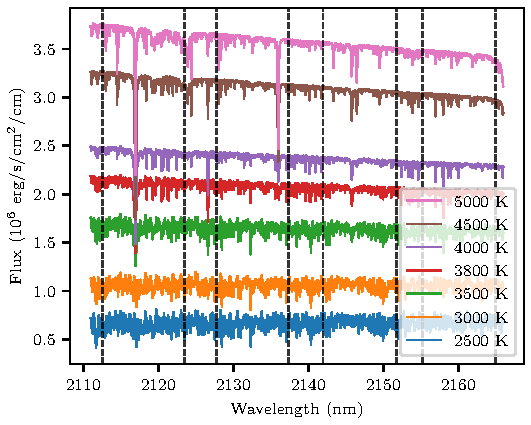
\includegraphics[width=\hsize]{./figures/companion_recovery/companion_spectra.pdf}
    \caption{{PHOENIX-ACES} spectra for temperatures between 2500 and 5000\K{}, corresponding to to the same lines in \cref{fig:injection_shape}.
The flux units are the native units of the {PHOENIX-ACES} spectrum, (\(\rm erg\,s^{-1}\,cm^{2}\,cm^{-1}\)), and have not been scaled by the stellar radii.
All spectra have a \Logg{}=5.0 and \feh{}=0.0.
The vertical dotted lines indicate the edges of the CRIRES detectors.}
    \label{fig:comp_spectra}
\end{figure}

\subsection{Component {RV} separation}
\label{subsec:rv_seperation}
Another factor which could contribute to an unsuccessful detection is the {RV} separation between the host and companion, is \Rvtwo{}.
Estimates for the observations are given in the last column of \cref{tab:observations}.
If \Rvtwo{} is small compared to the line width, then all the same lines of both components will be blended.
For example, \citep{kolbl_detection_2015} have difficultly separating blended spectra which have a component {RV} separation below 10\kmps{}.
This is indeed the case for {HD~4747}, {HD~211847}, and {HD~202206} with expected \(|\rvtwo{}| < 2\)\kmps{}.
This may have contributed to the lack of recovery with both components of the binary model trying to fit to the same features.
This may even cause some correlation between the parameters of the two components.
The {RV} separation of the two components changes with orbital phase.
Having multiple spectra of the same target distributed in phase may allow the {RV} of the spectral components to be better recovered~\citep [e.g.][]{czekala_disentangling_2017, sablowski_spectral_2016, piskorz_evidence_2016}.


\subsection {Wavelength range}
\label{subsec:wavelenght_range_limitation}
The wavelength choice for the spectra analysed here, observed with the intention to apply the spectral differential technique, was selected due to the location of the \emph{K}-band telluric absorption window.
This wavelength range, with a narrow wavelength range \(\sim\)50\nm{} set by the CRIRES instrument.
This wavelength range is not the best choice for the techniques applied here.

For instance~\citet{passegger_fundamental_2016} used four different spectral regions for the precise parameter determination of M-dwarfs using \textchisquared{} methods.
Specific lines in the different wavelength regions are affected differently by the model parameters: \Teff{}, \Logg{}, and \feh{}; and are used to break degeneracies in the {PHOENIX-ACES} parameter space.

Changing the wavelength coverage to regions with lines sensitive to stellar parameters for both stars and {BD}s, as well as using a larger wavelength range that will be achieved by {CRIRES+}, may help to improve the recovery results of the companion recovery technique presented here.

Several works \citet[e.g.][]{brogi_carbon_2014, brogi_rotation_2016, piskorz_evidence_2016} have had successful molecule and companion detections in the wavelength range around 2300\nm{} due to strong \ce{CO} lines.
This wavelength region has already been shown to be promising for simulations of the differential technique in~\citet{kostogryz_spectral_2013}.
This is clearly one wavelength region in particular to focus attention in the future.


\subsection{The {BT-Settl} models}
\label{subsec:bt-settl}
The {PHOENIX-ACES} models were not the only spectral libraries available with the other notable library considered for this work being the {BT-Settl} models~\citep{allard_model_2010,allard_btsettl_2013,baraffe_new_2015} (see \cref{subsec:btsettl}).

As the {BT-Settl} models are suitable to model the atmospheres of the brown dwarfs they would have been useful for the companion recovery technique developed here.
However, as shown in \cref{subsection:results-hd211847, subsection:injection-recovery}, a successful recovery of the 155\Mjup{} (\Teff{}\(\sim\)3200\K{}) low mass star companion of {HD~211847} was not possible.
Limiting the temperature and derived a temperature upper limit for \textrm{our} methodology of around 3800\K{}.
These are both well above the 2300\K{} cut-off of the {PHOENIX-ACES} models and for the onset of dust- and cloud-formation phenomena, at 2600\K{}.

As shown in \cref{subsec:phoenix_comparision} the {PHOENIX-ACES} and {BT-Settl} spectra are fairly similar.
\cref{fig:hd211847-models} shows again the minimum \textchisquared{} solution for detector \#1 of the second {HD~211847} observation, this time including the {BT-Settl} solution with the same parameters.
Although the {PHOENIX-ACES} and {BT-Settl} models differ slightly they both have large spectral discrepancies to the observations.
As such the {BT-Settl} models were not used in the \textchisquared{} simulations and results as there did not seem to be any special advantage in using them.
If promising results had been obtained with the {PHONEIX-ACES}, or a substantial difference between the synthetic spectral models more focus on the {BT-Settl} models would have occurred.


\begin{figure}
    \centering
    %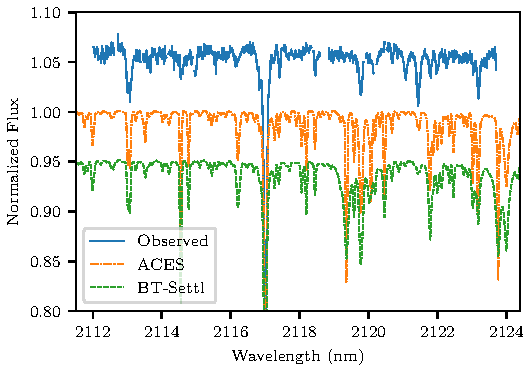
\includegraphics[width=\hsize]{images/final/HD211847_ACES_BTSettl.pdf}
    \caption{Detector \#1 spectrum for {HD~211847} (blue) alongside the {PHOENIX-ACES} (orange dash-dot) and {BT-Settl} (green dashed) synthetic spectra for the host star only, with parameters \Teff{}=5700\K{}, \Logg{}=4.5 and \feh{}=0.0.
        Both synthetic models have been normalized and convolved to \(\rm R=50\,000\).
        There is a 0.05 off-set between each spectrum}
    \label{fig:hd211847-models}
\end{figure}


\subsection{Impact of \Logg{}}
\label{subsec:logg} 
The surface gravity of a star, measured as \Logg{}, is related to evolutionary state and the size of the star.
Smaller \Logg{} values usually indicate bigger stars with larger radii.
This parameter has a large impact on the radius and thus flux ratio of the binary models.
In experimenting with the \Logg{} value of the {PHOENIX-ACES} models a decrease in \Logg{} from 5.0 to 4.5 increases the models effective radius by \(\sim\)1.75 in the temperature range investigated here.
This change in radius alone roughly triples the absolute flux of the synthetic spectrum (\(1.75^2\)), neglecting any changes to the shape of the actual spectrum.
Therefore, there are large jumps in the model flux ratios, and the \textchisquared{} solutions if the \Logg{} is allowed to vary.
Like with higher companion temperatures, a lower \Logg{} value for the companion is favoured as the increased flux ratio reduces the spectral mismatch of the host component to the observations.
This large impact of \Logg{} on the spectral library absolute flux is one reason for keeping the \Logg{} of each component fixed in the \textchisquared{} results presented in \cref{sec:chi2_results}.

\subsection{Interpolation}
\label{subsec:interpolation}
One procedure not incorporate into this \textchisquared{} procedure is spectral interpolation in between spectral grid points.
It is common to interpolate between the synthetic spectral grids to fit and derive parameters in between the grid points such as performed in~\citet{nemravova_xtauri_2016} and \citet{passegger_fundamental_2016}.
At a more advanced stage, instead of interpolation,~\cite{czekala_constructing_2015} use a spectral emulator and use Principal Component Analysis to create eigenspectra for the synthetic library and Gaussian processes to derive a probability distribution function of possible interpolation spectra to account for uncertainties in the interpolation required for high signal-to-noise spectra.

Interpolation could be something to be added to this work in the future to refine the recovered parameters, and to help the transition between the grid \Logg{} values.
Codes are readily available to perform spectral interpolation which could be utilized for this, two of them are \emph{pyterpol}\footnote{https://github.com/chrysante87/pyterpol}~\citet{nemravova_xtauri_2016} and \emph{Starfish}\footnote{https://github.com/iancze/Starfish}~\cite{czekala_constructing_2015}.


\subsection{Contrast to other works}

In this work the techniques attempted were unsuccessful in detecting the companions.
Here some relevant comparisons are made to recent positive detections in the literature.

\citet{passegger_fundamental_2016} apply \textchisquared{} fitting of M-dwarf spectra in the \nir{} to {PHOENIX-ACES} models, incorporating inter-grid interpolation to determine M-dwarf parameters.
Reaching a level inherent uncertainties on the parameters of \({\sigma}_{\teff}= 35\)\K{}, \({sigma}_{\logg{}} = 0.14\), and \({\sigma}_{\feh{}}= 0.11\), on four stars.
\citet{passegger_carmenes_2018} further extend this method to the 300 stars of the {CARMENES} library with optical and \nir{} spectra, achieving uncertainties of \({\sigma}_{\teff{}}=51\)\K{}, \({\sigma}_{\logg{}}=0.07\) and \({\sigma}_{\feh{}}\)=0.16.
The temperatures recovered are in line with the literature values while their metallicity determination has a larger spread when compared to the literature.
These uncertainties are much smaller than the library grid spacing due to the fine-grid search achieved by interpolation.
\citet{rajpurohit_exploring_2018} perform similar parameter determination, using the recent {BT-Settl} models instead, exploring more lower temperature M-dwarfs than \citet{passegger_carmens_2018}, at which point dust clouds begin to form.
The results of \citet{rajpurohit_exploring_2018} are in agreement with \citep{gadios_dwarf_2014} but they find a disagreement to the \citet{passegger_carmens_2018} parameters, particularly \Teff{}, with up to a 200--300\K{} difference between the {PHOENIX-ACES} and {BT-Settl} results.
Differences are also observed between the \Logg{} and \feh{} recovered by the two works.
Both these works, use a much larger wavelength range (\(\sim\)500--1700\nm{}) than utilized here.


In trying to detect secondary stellar spectra in optical spectra at \(R=60\,000\), \citep{kolbl_detection_2015} are able to detect secondary spectra down to a 1\% flux ratio, by matching to a library of real spectra.
The work performed here aimed at flux ratios starting around below this limit, even after taking advantage of the increased flux ratio in the \nir{}.


One promising technique with a success in detecting faint companion emission spectra is presented by \citet{lockwood_nearir_2014}.
Applying the {TODCOR} correlation to several spectra at different epochs and combining the observations while accounting for the orbits using a maximum likely-hood framework.
They confirm the water emission signature in {\(\tau\) Bootis} and find a \(1\sigma\) upper limit high resolution (\(R=24\,000\)) spectroscopic flux ratio of \(10^{-4}\) at 3.3\um{}.

\citep{piskorz_evidence_2016} used this same technique to achieve a detection of a non-transiting hot gas giant {HD~88133}b, with a flux ratio near \(10^{-5}\).
This is achieved with spectra from nine epochs, six in the\emph{L}-band and three epochs in the \emph{K}-band with the Keck {NIRPSEC} instrument (R= 25\,000--30\,000).
Each epoch has a combined exposure time of 60--180 minutes reaching a \snr{} between 1600--3000 allowing for the planetary emission spectra to be recovered around a flux ratio of \(10^{-5}\).

These successful works clearly reveal the difficultly faced with the spectra analysed in this current work.
Particularly, the \snr{} in \citep{piskorz_evidence_2016} is an order of magnitude higher and the wavelength coverage is significantly larger, due to the cross-dispersion of {NIRPSEC}.
Also the multi-epoch approach allows for the {RV} of the two components to be monitored and some orbital parameters determined.
The narrow wavelength coverage CRIRES spectra analysed here, at \snr{}=100--300 are insufficient.
The poorly separated epochs, were also a problem as addressed in \cref{subsec:differential_results}.


